%!TEX encoding = UTF-8 Unicode
%!TEX root = ../algos-geometriques.tex


\chapter{Oblong}

Un oblong est un rectangle terminé par deux demi-cercles :

\begin{center}
  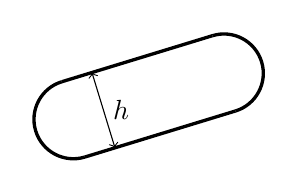
\begin{tikzpicture}[rotate=17]
    \draw[very thick] (0, 0) -- ++ (2, 0) ;
    \draw[very thick] (0, 1) -- ++ (2, 0) ;
    \draw[very thick] (2, 0) arc (-90:90:.5) ;
    \draw[very thick] (0, 0) arc (90:-90:-.5) ;
    \draw[thin, <->] (0.4, 0) -- ++ (0, 1) node[midway, right] {$h$} ;
  \end{tikzpicture}
\end{center}

Un oblong est défini par deux points et la hauteur de la partie centrale, qui est aussi le diamètre des cercles d'extrémité :

\begin{center}
  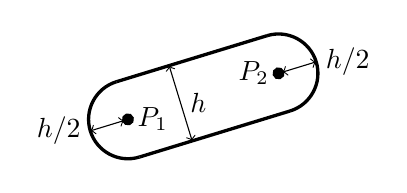
\begin{tikzpicture}[rotate=17]
    \draw[very thick] (0, 0) -- ++ (2, 0) ;
    \draw[very thick] (0, 1) -- ++ (2, 0) ;
    \draw[very thick] (2, 0) arc (-90:90:.5) ;
    \draw[very thick] (0, 0) arc (90:-90:-.5) ;
    \draw[fill] (0, 0.5) circle (2pt) node[right] {$P_1$} ;
    \draw[fill] (2, 0.5) circle (2pt) node[left] {$P_2$} ;
    \draw[thin, <->] (0.7, 0) -- ++ (0, 1) node[midway, right] {$h$} ;
    \draw[thin, <->] (2.05, 0.5) -- ++ (0.45, 0) node[right] {$h/2$} ;
    \draw[thin, <->] (-0.05, 0.5) -- ++ (-0.45, 0) node[left] {$h/2$} ;
  \end{tikzpicture}
\end{center}


\begin{lstlisting}
struct CanariOblong {
  let p1 : CGPoint
  let p2 : CGPoint
  let height : CGFloat

  init (from p1 : CGPoint, to p2 : CGPoint, height : CGFloat) {
    self.p1 = p1
    self.p2 = p2
    self.height = height
  }
  ...
}
\end{lstlisting}




\section{Point dans un oblong}

Il suffit de tester successivement si :
\begin{itemize}
  \item le point est dans le cercle de centre $P_1$ ;
  \item le point est dans le cercle de centre $P_2$ ;
  \item le point est dans le rectangle formé par la partie centrale ;
\end{itemize}

\begin{lstlisting}
  func contains (point p : CGPoint) -> Bool {
  //--- p inside P1 circle
    var inside = CGPoint.distance (self.p1, p) <= (height / 2.0)
  //--- p inside P2 circle
    if !inside {
      inside = CGPoint.distance (self.p2, p) <= (height / 2.0)
    }
  //--- p inside rectangle
    if !inside {
      let r = CanariRect (from: self.p1, to: self.p2, height: self.height)
      inside = r.contains (point: p)
    }
    return inside
  }
\end{lstlisting}










\section{Intersection avec un autre rectangle}

Il suffit de tester successivement si :
\begin{itemize}
  \item l'autre rectangle intersecte le cercle de centre $P_1$ ;
  \item l'autre rectangle intersecte le cercle de centre $P_2$ ;
  \item l'autre rectangle intersecte le rectangle formé par la partie centrale ;
\end{itemize}

\begin{lstlisting}
  func intersects (rect : CanariRect) -> Bool {
  //--- rect intersects P1 circle
    let c1 = CanariCircle (center: self.p1, radius: self.height / 2.0)
    var intersects = rect.intersects (circle: c1)
  //--- rect intersects P2 circle
    if !intersects {
      let c2 = CanariCircle (center: self.p2, radius: self.height / 2.0)
      intersects = rect.intersects (circle: c2)
    }
  //--- rect intersects rectangle
    if !intersects {
      let r = CanariRect (from: self.p1, to: self.p2, height: self.height)
      intersects = rect.intersects (rect: r)
    }
    return intersects
  }
\end{lstlisting}






\section{Dessiner}

Pour dessiner un oblong, le plus simple est de tracer le segment $P_1P_2$, avec l'épaisseur \texttt{height}. En précisant la terminaison \texttt{kCALineCapRound}, les deux demi-disques sont ajoutés au tracé. Si les points sont confondus, le tracé résulte en un disque.

\begin{lstlisting}
  func shape () -> CAShapeLayer {
    let mutablePath = CGMutablePath ()
    mutablePath.move (to: self.p1)
    mutablePath.addLine (to: self.p2)
    let newLayer = CAShapeLayer ()
    newLayer.path = mutablePath
    newLayer.lineWidth = self.height
    newLayer.lineCap = kCALineCapRound
    return newLayer
  }
\end{lstlisting}


Pour le tracé effectif, il faut préciser sa couleur, par exemple :
\begin{lstlisting}
    let oblong = CanariOblong (...)
    let shapeLayer = oblong.shape ()
    shapeLayer.strokeColor = NSColor.black.cgColor
\end{lstlisting}








\section{Point dans un oblong, autre méthode}

{\bf Cette technique n'est pas implémentée dans ElCanari.}

\begin{center}
  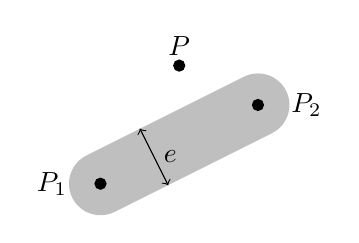
\begin{tikzpicture}
    \draw[line width=8mm, draw=lightgray, line cap=round] (0, 0) -- (2, 1) ;
%    \draw[thick] (0, 0) -- (2, 1) ;
    \draw[fill] (0, 0) circle (2pt) ;
    \draw[fill] (2, 1) circle (2pt) ;
    \draw[left] (-.3, 0) node {$P_1$} ;
    \draw[above] (1, 1.5) node {$P$} ;
    \draw[fill] (1, 1.5) circle (2pt) ;
    \draw[right] (2.3, 1) node {$P_2$} ;
    \draw[<->] (0.5, .7) -- ++ (0.36, -0.72) node[midway, right] {$e$} ;
  \end{tikzpicture}
\end{center}

Il y a un cas particulier si les deux points sont confondus : il suffit alors de calculer la distance entre $P$ et le point $P_1$ (ou $P_2$), et de la comparer avec $e/2$ ; ce n'est pas vraiment un cas particulier cas le cas général commence par tester si point $P$ dans le disque autour des extrémités.

Pour le cas général, on effectue trois tests :
\begin{itemize}
 \item point $P$ dans le disque autour de $P_1$ : calcul de la distance entre $P$ et $P_1$, et comparaison avec $e/2$ ;
 \item point $P$ dans le disque autour de $P_2$ : calcul de la distance entre $P$ et $P_2$, et comparaison avec $e/2$ ;
 \item point $P$ dans la partie centrale : c'est le plus compliqué, et est présenté ci-après. 
\end{itemize}

On considère le point $H (H.x, H.y)$, projection de $P$ sur $P_1P_2$.

\begin{center}
  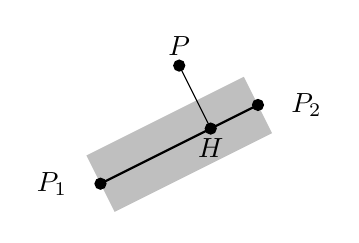
\begin{tikzpicture}
    \draw[line width=8mm, draw=lightgray, line cap=butt] (0, 0) -- (2, 1) ;
    \draw[thick] (0, 0) -- (2, 1) ;
    \draw[fill] (0, 0) circle (2pt) ;
    \draw[fill] (2, 1) circle (2pt) ;
    \draw[left] (-.3, 0) node {$P_1$} ;
    \draw[above] (1, 1.5) node {$P$} ;
    \draw[fill] (1, 1.5) circle (2pt) ;
    \draw[right] (2.3, 1) node {$P_2$} ;
    \draw (1, 1.5) -- (1.4, .7) ;
    \draw[fill] (1.4, .7) circle (2pt) ;
    \draw[below] (1.4, .7) node {$H$} ;
  \end{tikzpicture}
\end{center}

Le point $P$ est dans la partie centrale si et seulement si :
\begin{itemize}
  \item le point $H$ est entre $P_1$ et $P_2$ ;
  \item la distance $PH$ est inférieure à $e/2$.
\end{itemize}

Nous allons calculer les coordonnées de $H$, que l'on écrit sous la forme :

\begin{equation*}
h.x = \frac{p_1.x + p_2.x}{2} - \lambda ~ \frac{p_1.x - p_2.x}{2}\text{~et~}
h.y = \frac{p_1.y + p_2.y}{2} - \lambda ~ \frac{p_1.y - p_2.y}{2}
\end{equation*}

Ceci assure que $H$ est sur la droite $P_1P_2$ ; si $|\lambda|\leqslant1$, $H$ est entre $P_1$ et $P_2$. Pour calculer $\lambda$, on va écrire que $\overrightarrow{PH}$ et $\overrightarrow{P_1P_2}$ sont orthogonaux.

Ainsi :

\begin{equation*}
  \begin{array}{r|l}
    \overrightarrow{HP}
  &
    \begin{array}{l}
      \displaystyle\frac{p_1.x + p_2.x}{2} - \lambda ~ \frac{p_1.x - p_2.x}{2} - p.x
    \\
      \displaystyle\frac{p_1.y + p_2.y}{2} - \lambda ~ \frac{p_1.y - p_2.y}{2} - p.y
    \end{array}
  \end{array}
\end{equation*}

\begin{equation*}
  \begin{array}{r|l}
    \overrightarrow{P_2P_1}
  &
    \begin{array}{l}
       p_1.x - p_2.x
    \\
       p_1.y - p_2.y
    \end{array}
  \end{array}
\end{equation*}

Pour que ces deux vecteurs soient orthogonaux :

\begin{equation*}
 (\displaystyle\frac{p_1.x + p_2.x}{2} - \lambda ~ \frac{p_1.x - p_2.x}{2} - p.x) ~ (p_1.x - p_2.x) = 
 (\displaystyle\frac{p_1.y + p_2.y}{2} - \lambda ~ \frac{p_1.y - p_2.y}{2} - p.y) ~ (p_1.y - p_2.y)
\end{equation*}

D'où :

\begin{equation*}
\lambda = \frac{(p_1.x + p_2.x - 2~p.x)(p_1.x - p_2.x) + (p_1.y + p_2.y - 2~p.y)(p_1.y - p_2.y)}{(p_1.x - p_2.x)^2 + (p_1.y - p_2.y)^2} = \frac{N}{D}
\end{equation*}


\begin{lstlisting}
func segment (from p1 : CGPoint,
              to p2 : CGPoint,
              halfWidth : CGFloat,
              contains p : CGPoint) -> Bool {
//--- Near First point ?
  var contains = p.distanceTo (point: CGPoint (x: p1.x, y: p1.y)) < halfWidth
//--- Near Second point ?
  if !contains {
    contains = p.distanceTo (point: CGPoint (x: p2.x, y: p2.y)) < halfWidth
  }
//--- In segment ?
  if !contains && (( p1.x != p2.x) || (p1.y != p2.y)) {
    let dx = p1.x - p2.x
    let dy = p1.y - p2.y
    let N = (p1.x + p2.x - 2.0 * p.x) * dx + (p1.y + p2.y - 2.0 * p.y) * dy
    let D = dx * dx + dy * dy
    let lambda = N / D
    contains = abs (lambda) < 1.0
    if contains {
      let hx = (p1.x + p2.x) * 0.5 - lambda * dx * 0.5
      let hy = (p1.y + p2.y) * 0.5 - lambda * dy * 0.5
      contains = p.distanceTo (point: CGPoint (x: hx, y: hy)) < halfWidth
    }
  }
  return contains
}
\end{lstlisting}









\section{Distance d'un point à une droite, 3\up{e} méthode}


\begin{center}
  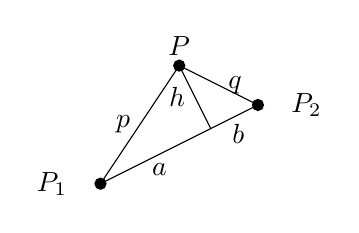
\begin{tikzpicture}
    \draw (0, 0)
       -- (1.5, 0.75) node[midway, below] {$a$}
       -- ++ (0.5, 0.25)  node[midway, below] {$b$}
       -- (1, 1.5) node[midway, right] {$q$}
        -- (0, 0) node[midway, left] {$p$} ;
    \draw (1, 1.5) -- ++ (0.4, -0.8) node[midway, left] {$h$} ;
    \draw[fill] (0, 0) circle (2pt) ;
    \draw[fill] (2, 1) circle (2pt) ;
    \draw[left] (-.3, 0) node {$P_1$} ;
    \draw[above] (1, 1.5) node {$P$} ;
    \draw[fill] (1, 1.5) circle (2pt) ;
    \draw[right] (2.3, 1) node {$P_2$} ;
  \end{tikzpicture}
\end{center}

Problème : connaissant les trois points $P_1$, $P_2$ et $P$, calculer $h$. Plus présicement, on connait :
\begin{itemize}
  \item $p$, distance entre $P_1$ et $P$ ;
  \item $q$, distance entre $P_2$ et $P$ ;
  \item $d = a + b$, distance entre $P_1$ et $P_2$.
\end{itemize}

Le système est donc (où les inconnues sont $a$, $b$ et $h$, on cherche $h$) :
\begin{equation*}
  \begin{array}{r}
    d = a + b \\
    p^2 = a^2 + h^2 \\
    q^2 = b^2 + h^2
  \end{array}
\end{equation*}

Il vient :
\begin{equation*}
 p^2 - q^2 = a^2 - b^2 = (a + b) (a- b) = d (a - b)
\end{equation*}

Donc (ce qui exige que les deux points $P_1$ et $P_2$ soient distincts) :
\begin{equation*}
 a - b = \frac{p^2 - q^2}{d}
\end{equation*}

D'autre part :
\begin{equation*}
 2 h^2 = p^2 + q^2 - a^2 - b^2 = p^2 + q^2 - \frac{1}{2} (a+b)^2 - \frac{1}{2} (a-b)^2
\end{equation*}

Finalement :
\begin{equation*}
 4 h^2 = 2 p^2 + 2 q^2 -d^2 - (\frac{p^2 - q^2}{d})^2
\end{equation*}

